\documentclass[twocolumn]{ujarticle}

\setlength{\topmargin}{-2.0cm}
\setlength{\oddsidemargin}{-0.8cm}
\setlength{\evensidemargin}{-0.8cm}
\setlength{\textheight}{25.5cm}
\setlength{\textwidth}{18cm}
\setlength{\columnsep}{1cm}

\usepackage{amsmath}
\usepackage{amssymb}
\usepackage{amsthm}
\usepackage{eucal}
\usepackage[dvipdfmx]{graphicx}
\usepackage[dvipdfmx, hidelinks]{hyperref}
\usepackage[capitalize]{cleveref}
\usepackage{tikz}
\usetikzlibrary{calc}

\newcommand{\tikzinline}[2][3em]{
  \resizebox{!}{#1}{#2}
}

\renewcommand{\figurename}{Figure}
\DeclareMathOperator{\Hom}{Hom}
\newcommand{\ZZ}{\mathbb{Z}}
\newcommand{\QQ}{\mathbb{Q}}
\newcommand{\RR}{\mathbb{R}}
\newcommand{\NN}{\mathbb{N}}
\newcommand{\boxprod}{\mathbin{\square}}

\newcommand{\graphimg}[2][]{
  \includegraphics[#1]{Tikz/Graphs/out/#2}
}
\newcommand{\mathgraph}[2][3em]{
  \resizebox{!}{#1}{\graphimg{#2}}
}

\newcommand{\TITLE}
{The magnitude of graphs and the magnitude homology as its categorification}
\newcommand{\STNO}
{2264257}
\newcommand{\NAME}
{谷内 賢翔}
\newcommand{\ADVR}
{野崎 雄太 准教授}
\newcommand{\DATE}
{(2026年2月6日)}
\newcommand{\NENDO}
{2025年度}

\makeatletter
\def\ps@lrheadf{\ps@empty
  \def\@evenhead{\normalfont
      \leftmark{}{}\hfil \rightmark{}{}}
  \let\@oddhead\@evenhead
  \def\@oddfoot{}
  \let\@evenfoot\@oddfoot
  \let\@mkboth\markboth}
\makeatother

\pagestyle{lrheadf}

\markboth{
2025 年度 数物・電子情報系学科 数理科学 EP 卒業研究 概要
}{}


\begin{document}
\fontsize{9pt}{13pt}\selectfont


\twocolumn[
\centering
\textbf{\Large \TITLE}

\vskip5pt
\hfil 
{\large \STNO \hskip1zw \NAME
\hskip 2zw Supervisor : \ADVR}

\vskip15pt

]

\noindent
\textbf{1. 研究背景・動機}

The concept of magnitude was introduced by Leinster [2] and it is defined for enriched categories of finite objects such as generalized metric spaces. For example, given a finite graph $G$, let $X_G$ be the generalized finite metric space consisting of vertices of $G$ equipped with the shortest path metric. Subsequently, Leinster focuses on the magnitude of graphs in [3] using the idea of magnitude of a metric space. Some properties of magnitude are multiplicativity with respect to cartesian product, denoted by $\boxprod$, and an inclusion-exclusion formula for the magnitude of a union under mild hypotheses:
\[
  \# (G \boxprod H)=\# G \cdot \# H, \quad \# (G \cup H) = \# G + \# H - \#(G \cap H).
\]
For example, the magnitude of the Cartesian product of the complete graph on 2 vertices $K_2$ and that on 3 vertices $K_3$ satisfies:

\[
  \# \tikzinline[1.5em]{
    \begin{tikzpicture}[
      baseline=(current bounding box.center),
      vertex/.style={circle, fill=black, inner sep=0pt, minimum size=18pt},
      edge/.style={thick},
      hidden edge/.style={thick, dashed, gray}
    ]
    \coordinate (B1) at (0, 1);
    \coordinate (B2) at (2.5, 1);
    \coordinate (B3) at (1.25, -0.5);
    \coordinate (T1) at ($(B1)+(0, 3)$);
    \coordinate (T2) at ($(B2)+(0, 3)$);
    \coordinate (T3) at ($(B3)+(0, 3)$);
    \draw[edge] (B1) -- (B2);
    \draw[edge] (B1) -- (B3) -- (B2);
    \draw[edge] (B1) -- (T1);
    \draw[edge] (B2) -- (T2);
    \draw[edge] (B3) -- (T3);
    \draw[edge] (T1) -- (T2) -- (T3) -- cycle;
    \foreach \v in {B1, B2, B3, T1, T2, T3} {
      \node[vertex] at (\v) {};
    }
    \end{tikzpicture}
  }
  = 
  \# \tikzinline[1em]{
    \begin{tikzpicture}[baseline=(current bounding box.center)]
        \coordinate (A) at (0, 0);
        \coordinate (B) at (0, 0.5);
        \draw[thick] (A) -- (B);
        \fill (A) circle (2pt);
        \fill (B) circle (2pt);
    \end{tikzpicture}
  }
  \cdot 
  \# \tikzinline[1em]{
    \begin{tikzpicture}[baseline=(current bounding box.center)]
        \coordinate (A) at (0.5, 0.866);
        \coordinate (B) at (0, 0);
        \coordinate (C) at (1, 0);
        \draw[thick] (A) -- (B) -- (C) -- cycle;
        \fill (A) circle (2pt);
        \fill (B) circle (2pt);
        \fill (C) circle (2pt);
    \end{tikzpicture}
  }
\]


Formally, the magnitude of a graph is defined to be a rational function over $\QQ$. Since the distance on a graph takes value in integers, it can also be expressed as a formal power series over $\ZZ$.

Hepworth and Willerton introduced a bigraded homology theory for graphs in [1], which has the magnitude as its graded Euler characteristic, and showed how properties of magnitude proved by Leinster categorify to properties such as a K\"{u}nneth Theorem and a Mayer-Vietoris Theorem.

Here, we focus on the inclusion-exclusion formula and the relation between the magnitude of graphs and that of enriched categories. We denote the magnitude of a graph $G$ by $\# G$ and the magnitude homology of $G$ by $MH_{*,*}(G)$.

\vskip10pt
\noindent
\textbf{2. 主結果}

The first main result establishes the inclusion-exclusion formula, a fundamental property for graph invariants;
\[
  \# (G \cup H) = \# G + \# H - \#(G \cap H).
\]
For this we must impose some hypotheses. Indeed, Leinster [3] shows that there is no nontrivial graph invariant that is fully cardinality-like in the sense of satisfying both multiplication and inclusion-exclusion formula without restriction. However, the hypotheses we impose are mild enough to cover a wide range of examples, including trees, forests, wedge sums, and certain graphs containing a cycle of length at least 4 (for example, see Figure \ref{fig:connect_c4}).
\begin{figure}[htbp]
    \centering
    \graphimg[width=0.5\linewidth]{connect_C_4.pdf}
    \caption{The graph containing a cycle of length 4}
    \label{fig:connect_c4}
\end{figure}

The second main result confirms that the magnitude defined in the context of enriched categories coincides with that defined in the context of graphs.


\vskip10pt
\noindent

\textbf{3. 意義・証明のアイデア}

The significance of this research lies in establishing an effective inclusion-exclusion formula for the magnitude of graphs and clarifying its categorical foundation.

For the first main result regarding the inclusion-exclusion formula, the core idea of the proof is to construct the weighting $w_X$ for $X$ linearly as $w_X = w_G + w_H - w_{G \cap H}$.
The validity of this construction relies on the metric property induced by the projection $\pi: V(H) \to V(G \cap H)$. Specifically, the projection condition ensures the metric equality
$d(g, h) = d(g, \pi(h)) + d(\pi(h), h)$
for any $g \in V(G)$ and $h \in V(H)$. Using this equality, one can verify that the linear combination of weightings satisfies the weighting equation $\sum_{y \in V(X)} q^{d(x,y)}w_X(y) = 1$ for all $x \in V(X)$.

For the second main result connecting graphs to enriched categories, the proof proceeds as follows.
A finite graph $G$ is identified with a generalized metric space, which is structurally a $[0, \infty]$-enriched category. We define a map $|\cdot|$ by $|x| = q^x$. Since the distance function $d$ on a graph $G$ takes values in $\NN \cup \{\infty\}$, this map satisfies the properties required for a valuation on the enriched category.
Under this valuation, the similarity matrix of the category, defined by $\zeta(a,b) = |\mathrm{Hom}(a,b)|$, becomes exactly $q^{d_G(a,b)}$. Thus, the categorical definition of magnitude naturally recovers the graph magnitude defined by weighting vectors.

\textbf{4. 今後の課題}

Based on the results of this thesis, several open problems remain to be explored:
\begin{itemize}
    \item \textbf{Whitney Twist:} Leinster showed that if two graphs differ by a Whitney twist with adjacent gluing points, then their magnitudes are equal. Does this equality extend to an isomorphism of magnitude homology groups?
    \item \textbf{Diagonal Graphs:} Computations suggest that the icosahedral graph has diagonal homology (i.e., $MH_{k,l} = 0$ for $k \neq l$). Is there a general graph-theoretic characterization of diagonal graphs?
\end{itemize}

\vskip10pt
\noindent
\textbf{参考文献}

{\small
\noindent
[1] R. Hepworth and S. Willerton. \textit{Categorifying the magnitude of a graph}. Homology Homotopy Appl. 19 (2017), no. 2, 31-60.

\noindent
[2] T. Leinster. \textit{The magnitude of metric spaces}. Doc. Math. 18 (2013), 857-905.

\noindent
[3] T. Leinster. \textit{The magnitude of a graph}. Math. Proc. Cambridge Philos. Soc. 166 (2019), no. 2, 247-264.
}

\end{document}